\documentclass[12pt]{book}
\usepackage[utf8]{inputenc}				% поддержка UTF8
\usepackage[english,russian]{babel}  	% поддержки русского языка
\usepackage{listings}					% листинги с кодом
\usepackage{menukeys}					% кнопки клавиатуры
\usepackage[unicode, pdftex]{hyperref}	% гиперссылки
\usepackage{outlines}					% многоуровневые списки
\usepackage{indentfirst}				% первый абзац
\usepackage{cmap}       				% теперь из pdf можно копипастить русский текст
\usepackage{xcolor}
\usepackage{geometry}
\usepackage{tikz}

\setcounter{secnumdepth}{3}				% вложенность секций до третьего уровня

\usefont{T2A}{ftm}{m}{} % Ужирнение начертания шрифта --- после чего
% выглдяит таймсоподобно и удобнее для чтения
% в плохих условиях.

\geometry{verbose,a4paper,tmargin=2cm,bmargin=2cm,lmargin=2.5cm,rmargin=1.5cm}

\definecolor{codegreen}{rgb}{0,0.6,0}
\definecolor{codegray}{rgb}{0.5,0.5,0.5}
\definecolor{codepurple}{rgb}{0.58,0,0.82}
\definecolor{backcolour}{rgb}{0.95,0.95,0.92}

\lstdefinestyle{mystyle}{
	backgroundcolor=\color{backcolour},   
	commentstyle=\color{codegreen},
	keywordstyle=\color{magenta},
	numberstyle=\tiny\color{codegray},
	stringstyle=\color{codepurple},
	basicstyle=\ttfamily\footnotesize,
	breakatwhitespace=false,         
	breaklines=true,                 
	captionpos=b,                    
	keepspaces=true,                 
	numbers=none,                    
	numbersep=5pt,                  
	showspaces=false,                
	showstringspaces=false,
	showtabs=false,                  
	tabsize=2
}
\lstset{style=mystyle}


\begin{document}
	\tableofcontents
	
	%
% Определение новых команд используемых при написании документа, для единообразия оформления
%

\renewcommand{\cmd}[1]{% команда консоли
	\texttt{#1}
}

\newcommand{\opt}[2]{% опция команды
	\textbf{#1} -- #2
}   

\newcommand{\cfgfile}[1]{% конфигурационный файл или файл с настройками
	\textcolor{red}{#1}
}   

\newcommand{\cfgpath}[1]{% путь к настройкам или части системы
	\textcolor{blue}{#1}
}   

	\chapter{Введение}

Задача данной методички -- дать \textbf{практические навыки} работы в консоли Linux, на примере дистрибутива Debian. В методичке обозначаются основные команды, горячие клавиши, инструменты и варианты их использования, а так же методы быстрой и эффективной работы в консоли Linux. В то же время не уходя слишком далеко в детали, оставляя некоторые инструменты и темы открытыми, чтобы читатель провёл самостоятельное их изучение, посредством чтения оригинальной документации, поиска в \href{https://google.com}{Google}, изучения \href{https://stackoverflow.com}{StackOverflow} и просмотра \href{https://youtube.com}{YouTube}. Последнее менее желательно, т.к. концентрация полезной информации в единицу времени достаточно низкая, а качество и полнота преподносимой информации желает лучшего. Никакой сайт или обучающее видео не смогут сравниться с полнотой оригинальной документации, об этом нужно всегда помнить и акцентировать внимание при изучении \textbf{абсолютно любой} технологии, программы, языка программирования, методологии и т.п.

Умение читать оригинальную документацию на английском языке (по диагонали), при этом находя то что нужно -- является критически необходимым навыком, который нужно развивать для быстрой и эффективной работы, т.к. информации на английском языке всегда было и будет больше, в силу того, что мировое сообщество его выбрало в качестве общего для общения и совместной работой между специалистами разных стран. Так же зачастую информация на английском языке является единственным источником о конфигурировании тех или иных инструментов, поэтому умение читать и понимать технические тексты на английском языке является критически важным навыком для успешной работы в IT-сфере.
\\

\noindent \textbf{P.S.} Для единообразия описания, были приняты следующие обозначения и соглашения:

\begin{itemize}
	\item \keys{ Ctrl + X } -- нажатие сочетания клавиш Ctrl+X
	\item \cmd{pwd} -- команда консоли (программа)
	\item \argum{arg} -- аругмент/параметр команды
	\item \cfgfile{/etc/passwd} -- конфигурационный файл или файл с настройками
	\item \cfgpath{/proc/} -- путь к директории с файлами процессов
\end{itemize}

\noindent  \textbf{P.S.2.} В данном методическом пособии слово \textit{команда} употребляется, как синонимом слова \textit{программа} и по сути таковой и является, если речь не идёт о встроенных командах shell-оболочек таких как: \cmd{sh}, \cmd{bash}, \cmd{zsh}.

%\section{vi}
%\section{nano}
%\section{базовые команды}
%\section{регулярные выражения}
%\section{командая строка и bash}
%\section{экранные менеджеры screen, tmux}
%\section{философия unix}
%\section{иерархия файлов}

%\begin{figure}
	%\centering
%	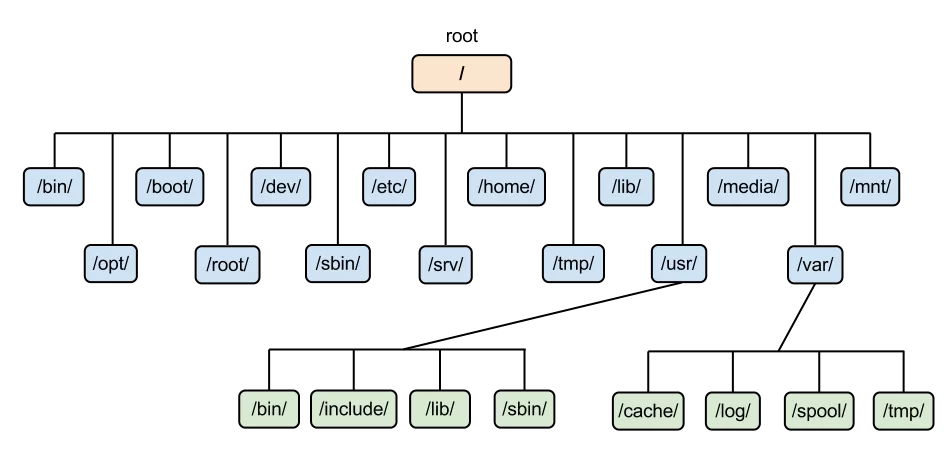
\includegraphics[width=\textwidth]{img/ch1/hfs.png}
%	\caption{Иерархия файловой системы}
%	\label{fig:galaxy}
%\end{figure}

%\keys{Сtrl + Shift + F}

%man -K IPX

%\texttt{man}

%\keys{Сtrl + Shift + F}

	
	\chapter{Основные команды}

	%\include{history}%философия unix
	%\include{promtcmd}%командая строка
	%\include{basecmd}базовые команды
%	\include{hfs}
	\section{man}

\cmd{man} - сокращение от manual, команда позволяет просматривать справочную информацию о программах Linux или командах shell-оболочки (\cmd{bash, sh, dash, zsh} и пр.), форматах конфигурационных файлов, специальных файлов устройств, описание системных вызовов или библиотечных вызовов и системных команд администратора. Пример формата вызова \cmd{man}:

\begin{lstlisting}
	
	$ man [section] page
	
\end{lstlisting}	

\begin{itemize}	
	\item \textit{section} тип страницы справочной информации:
	
	\subitem \opt{1}{программы или команды shell-оболочки}
	\subitem \opt{2}{системные вызовы (функции ядра: fork, accept, listen, select, mmap и пр.)}
	\subitem \opt{3}{библиотечные вызовы (функции библиотек: fopen, pow, malloc и пр.)}
	\subitem \opt{4}{специальные файлы (обычно находящиеся в \cfgpath{/dev/}: random, mem, tty и пр.)}
	\subitem \opt{5}{форматы файлов (\cfgfile{/etc/passwd}, \cfgfile{/etc/shadow},  \cfgfile{$\sim$/.ssh/authorized\_keys} и пр.)}
	\subitem \opt{6}{игры}
	\subitem \opt{7}{описания, соглашения и пр.}
	\subitem \opt{8}{команды системного администратора (доступные только для root и/или sudo-пользователя: \cmd{ss, adduser, sysctl} и пр.)}

	\item \textit{page} имя программы, команды, конфигурационного файла, системного вызова и т.д.
\end{itemize}

Посмотреть информацию о команде \cmd{man}:
\begin{lstlisting}
	
	$ man man
	
\end{lstlisting}

После входа в интерактивный режим \cmd{man} доступны следующие функции:

\noindent\keys{ q } -- выход из \cmd{man} (обратить внимание, чтобы раскладка была английской) \\
\keys{ h } -- посмотреть помощь по навигации \cmd{man} \\

\noindent\keys{ u } / \keys{ d } -- пролистать на пол экрана вверх/вниз \\
\keys{ y } или \keys{ \arrowkeyup } -- пролистать на одну строку вверх \\
\keys{ e } или \keys{ \arrowkeydown } -- пролистать на одну строку вниз \\
\keys{ w } / \keys{ PgUp } -- пролистать на один экран вверх\\
\keys{ z } / \keys{ PgDown } -- пролистать на один экран вниз\\
\keys{ g } / \keys{ G }  -- переместиться в начало/конец документа \\

\noindent\keys{ / } + \textit{ввести шаблон поиска} -- прямой поиск по шаблону\\
\keys{ ? } + \textit{ввести шаблон поиска} -- обратный поиск по шаблону\\
\keys{ n } / \keys{ N } -- повторить предыдущий поиск в прямом/обратном направлении\\

Для включения/отключения нумерации строк в режиме просмотра справочной страницы необходимо ввести соответствующие опции и нажать \keys{ Enter }:\\ 
\noindent
\opt{-N}{включить нумерацию строк}\\
\opt{-n}{выключить нумерацию строк}\\

Показать все доступные разделы справочной информации по \cmd{passwd}:
\begin{lstlisting}
	
	$ man -f passwd
	
\end{lstlisting}	


Показать раздел 1 справочной информации для команды \cmd{passwd}:
\begin{lstlisting}
	
	$ man 1 passwd
	
\end{lstlisting}	

Показать раздел 5 справочной информации о формате файла \cfgfile{/etc/passwd}:
\begin{lstlisting}
	
	$ man 5 passwd
	
\end{lstlisting}	

Поиск всех справочных страниц в названии или описании которых встречается \textit{ls}:
\begin{lstlisting}
	
	$ man -k ls
	
\end{lstlisting}	

Поиск по всем справочным страницам сочетания слов \textit{password change}:
\begin{lstlisting}
	
	$ man -K "password change"
	
\end{lstlisting}	
\keys{ Enter } -- открыть страницу из результата поиска\\
\keys{ Ctrl + D } -- пропустить страницу\\
\keys{ Ctrl + C } -- закрыть поиск\\

Просмотреть страницу справки команды \cmd{man} на русском языке (если страница справки с соответствующей русской локалью \textit{ru\_RU} имеется в системе):
\begin{lstlisting}
	
	$ man -L ru_RU man
	
\end{lstlisting}	

\noindent
\cfgfile{/etc/manpath.config} -- файл настройки man-db\\
\cfgpath{/usr/share/man/} -- здесь расположены файлы со справочными страницами\\

%	\include{bash}
	\section{nano}

\noindent
\cmd{nano} -- текстовый редактор. Чтобы создать новый файл с именем \argum{file} или открыть существующий в режиме редактирования, необходимо выполнить команду \footnote{(если параметр \argum{file} не указывать, то откроется редактор с пустым документом}:

\begin{lstlisting}
	
	$ nano file
	
\end{lstlisting}	

После открытия редактора \cmd{nano} \ref{fig:nano}, внизу можно увидеть следующие подсказками: \verb|^|\textbf{X} Exit, \verb|^|\textbf{G} Help и т.д. В *nix системах сочетения нажатия клавиши \keys{Ctrl} с нажатием другой клавиши обозначается, как символ \verb|^| и далее название клавиши, так нажатие сочетания клавиш \keys{Ctrl + X} и \keys{Ctrl + C} обозначаются, как \verb|^|\textbf{X} и \verb|^|\textbf{C} соответственно.

\begin{figure}[h]
\centering
	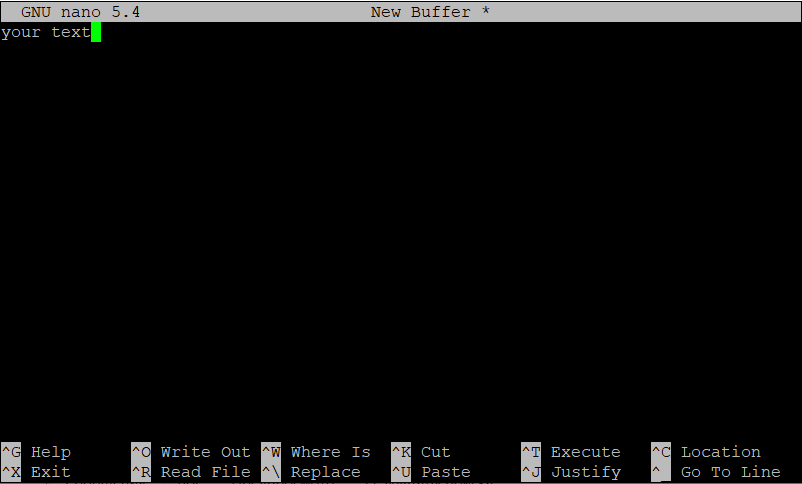
\includegraphics[width=\textwidth]{img/ch1/nano.png}
	\caption{Редактор \cmd{nano} после открытия}
	\label{fig:nano}
\end{figure}

Так же в \cmd{nano} можно открыть более одного файла одновременно, например:
\begin{lstlisting}
	
	$ nano file1 file2 file3
	
\end{lstlisting}	

В результате будут открыты файлы \argum{file1}, \argum{file2} и \argum{file3} в так называемый \textit{буфферах} (экраны, между которыми можно переключаться сочетаниями клавиш \keys{ Atl + > } и \keys{ Atl + < }). Так же можно набор файлов по маске, например:
\begin{lstlisting}
	
	$ nano *.log
	
\end{lstlisting}	

\noindent
\keys{ Ctrl + X } -- закрыть текущий буффер и выйти из \cmd{nano}\\
\keys{ Ctrl + O } -- сохранить изменение текущего буффера в файл\\
\keys{ Ctrl + R } -- открыть файл в текущем буфере\\
(\keys{ Ctrl + R })  + (\keys{ Atl + F }) -- открыть файл в новом буфере\\
(\keys{ Ctrl + R })  + (\keys{ Atl + F }) + (\keys{ Enter }) -- создать новый буффер\\


\noindent
{\large{Редактирование:}}\\
\keys{ Atl + A }/\keys{ Atl + 6 } -- выделить текст с текущей позиции курсора или отменить выделение\\
\keys{ Ctrl + 6 } -- скопировать выделенный текст\\
\keys{ Ctrl + K } -- вырезать текущую строку или выделенный текст в буфер обмена\\
\keys{ Ctrl + U } -- вставить содержимое буфера обмена в текущую позицию курсора\\
\keys{ Atl + M } -- вырезать от позиции курсора до конца файла\\
\keys{ Ctrl + D } -- удалить символ справа от курсора\\
\keys{ Ctrl + H } -- удалить символ слева от курсора\\
\keys{ Ctrl + M } -- вставить пустую строку\\
\keys{ Atl + R } -- заменить текст или регулярное выражение\\
\keys{ Ctrl + W } -- искать текст или регулярное выражение\\
\keys{ Atl + W } -- повторить последний поиск\\

\noindent
{\large{Навигация:}}\\
\keys{ PgUp }/\keys{ PgDown } -- пролистать на один экран вверх/вниз\\
\keys{ Ctrl  + }/\keys{ Atl + } -- вперёд/назад  на одно слово\\
\keys{ Atl + E }/\keys{ End } -- в конец текущей строки\\
\keys{ Atl + A }/\keys{ Home } -- в начало текущей строки\\
\keys{ Atl + $\setminus$}/\keys{ / }  -- на первую/последнюю строку файла\\
\keys{ Ctrl + \_ } -- перейти на указанный номер \textbf{строки} или \textbf{строки,позиции}\\

\noindent
{\large{Прочее:}}\\
\keys{ Atl + C } -- отображение положения курсора включить/отключить\\
\keys{ Ctrl + C } -- показать положение курсора (если в режиме редактирования документа)\\
\keys{ Atl + P } -- отображение пробелов\\
\keys{ Atl + Y } -- подсветка синтаксиса\\
\keys{ Atl + I } -- автоотступы\\
\keys{ Atl + H } -- умная клавиша HOME\\
\keys{ Atl + D } -- подсчитать количество слов, строк и символов в документе\\
\keys{ Atl + M } -- включить/отключить мышку для позиционирования курсора в редакторе\\
\keys{ Atl + N } -- включить/отключить нумерацию строк\\

Открыть файл \argum{file} и перейти к строке \textit{line} и столбцу \textit{col}:
\begin{lstlisting}
	
	$ nano +line,col <file>
	
\end{lstlisting}	

Открыть файл \argum{file} с нумерацией строк:
\begin{lstlisting}
	
	$ nano -l <file>
	
\end{lstlisting}	

Двойное нажатие \keys{Esc}, а затем ввод \textbf{трёхзначного числа} от \textbf{000} до \textbf{255} вставит символ с соответствующим ему hex-кодом.

Открыть файл \argum{file} предварительно сохранив его резервную копию:
\begin{lstlisting}
	
	$ nano -B <file>
	
\end{lstlisting}	

Чтобы указать директорию для сохранения резервных копий редактируемого файла или файлов, используется опция -C:
\begin{lstlisting}
	
	$ nano -BC <dir> <file>
	
\end{lstlisting}	


Открыть файл \argum{file} только для чтения используется ключ -v:
\begin{lstlisting}
	
	$ nano -v <file>
	
\end{lstlisting}	

	\section{vim}

\noindent
\cmd{vim} -- самый популярный текстовых редактор предустановленный на всех *nix-like системах, поэтому умение работать в нём является \textbf{обязательным}. Для ознакомления с базовой работой в \cmd{vim} можно воспользоваться встроеным мини-учебником \cmd{vimtutor}, который можно вызвать и командной строки. Чтобы запустить его русскую версию необходимо выполнить команду:

\begin{lstlisting}
	
	$ vimtutor ru
	
\end{lstlisting}	

В редакторе \cmd{vim} есть два режима работы:
\begin{itemize}
	\item \textbf{командный режим} -- чтобы в него перейnи необходимо нажать клавишу \keys{Esc}
	\item \textbf{режим ввода текста} -- чтобы в него перейти нужно нажать клавишу \keys{i}
\end{itemize}


\noindent
Создать или открыть файл с именем \argum{file} для редактирования \footnote{если параметр \argum{file} не указывать, то откроется редактор с пустым документом, сохранить который в дальнейшем возможно посредством ввода команды \textbf{:w} \argum{file} + \keys{Enter}}:

\begin{lstlisting}
	
	$ vi file
	
\end{lstlisting}	

После запуска \cmd{vim} редактор по умолчанию находится в \textbf{командном режиме} и в дальнейшем вся работа в редакторе строится посредством переключения между этими двумя режимами по мере необходимости и работе в каждом из них. В \textbf{командном режиме} вводить текст невозможно, но с помощью нажатия ряда клавиш (комбинации которых будут описаны ниже), возможно редактирование документа и навигация по нему. Стоит отметить, что в \textbf{командном режиме} при вводе команд они \textbf{не отображаются} на экране, за исключением команд, которые начинаются со специальных символов <<\textbf{:}>>, <<\textbf{/}>> или <<\textbf{?}>>. Если в же в \textbf{командном режиме} вводится команда и она начинается с символов <<\textbf{:}>>, <<\textbf{/}>> или <<\textbf{?}>>, в этом случае они отображаются в самой нижней строке экрана, она никак не связана с редактируемым документом и является \textbf{командной строкой} редактора \cmd{vim}. 

Если же необходимо вводить новые символы в документе или удалить посимвольно ранее набранный текст, то необходимо переключиться в \textbf{режим ввода текста} посредством нажатия клавиши \keys{i}, для всех остальных манипуляций с текстом в \cmd{vim} используется \textbf{командный режим}, в который можно перейти посредством нажатия клавиши \keys{Esc}.

\noindent
Открыть файл \argum{file} для просмотра:
\begin{lstlisting}
	
	$ view file
	
\end{lstlisting}	

\noindent
Открыть последнюю сохраненную версию файла \argum{file} после аварийного выхода:
\begin{lstlisting}

	$ vi -r file
	
\end{lstlisting}	

\noindent
Открыть файл \argum{file} и поместить курсор на последнюю строку \argum{n}:
\begin{lstlisting}
	
	$ vi +n file
	
\end{lstlisting}	

\noindent
Открыть файл \argum{file} и поместить курсор на последнюю строку:
\begin{lstlisting}
	
	$ vi + file
	
\end{lstlisting}	

\noindent
Открыть файл \argum{file} и поместить курсор на первое вхождение \argum{string}:
\begin{lstlisting}
	
	$ vi +/string file
	
\end{lstlisting}	

\noindent
Чтобы создать или открыть файл \argum{file} с использованием шифрования, необходимо выполнить команду, а далее ввести ключ для шифрования/дешифрования в зависимости от того создаётся ли файл или открывается уже шифрованный:

\begin{lstlisting}
	
	$ vi -x file
	
\end{lstlisting}	



\noindent
\keys{:} -- переход в режим \textbf{командной строки} \footnote{как таковой клавиши \keys{:} нет, для получения данного символа необходимо нажать сочетание \keys{Shift + ;} в английской расскладке клавиатуры, необходимо обратить на этот факт особое внимание, т.к. в дальнейшем, например, при указании например клавиши \keys{\$} подразумевается нажатие сочетания \keys{Shift + 4}, а при указании клавиши \keys{\_} подразумевается нажатие сочетания клавиш \keys{Shift + -} и т.д.}, не путать с \textbf{командным режимом}. Суть режима заключается в том, что после введения двоеточия, будучи в \textbf{командном режиме}, далее появляется возможность вводить ряд команд с целью управления документом и состоянием редактора в появившейся снизу командной строке, а так же навигации по списку введённых команд в \textbf{командной строке} в \cmd{vim}, посредством стрелок на клавиатуре \keys{ \arrowkeyup }/\keys{ \arrowkeydown }. Пример таких команд перечислен ниже:

\noindent
\opt{:q}{выход из текстового редактора \footnote{фактически это нажатие сочетания клавиш \keys{Shift+;} и далее нажатие \keys{q} и для выполнения команды нажать \keys{Enter}. Если набираемая команда выводится не снизу экрана в \textbf{командной строке} \cmd{vim}, то скорее всего текущий режим это \textbf{режим ввода текста}, необходимо перейти в режим \textbf{командной строки} посредстом нажатия \keys{Esc} и повторить ввод команды}}\\
\opt{:q!}{выход без сохранения}\\
\opt{:wq}{выход с сохранением}\\
\opt{:w}{сохранить файл или внесенные изменения}\\
\opt{:e}{загрузить файл для редактирования \footnote{после ввода команды ставится пробел и вводится имя файла, которое требуется закрузить или вводятся первые буквы названия файла и для \textbf{автодополнения} жмётся кнопка \keys{Tab} (иногда несколько раз, если есть несколько файлов, которые начинаются с указанных первых букв), пока не дополнит до искомого имени файла. Это всё работает, если файл находится в той же директории, в противном случае указывается путь к файлу и только в конце указывается требуемый файл. В процессе указания полного пути к файлу рекомендуется пользоваться автодополнением с помощью нажатия клавиши \keys{Tab}}}\\

\subsection*{Редактирование}
В \textbf{командном режиме} действуют следующие комбинации клавиш для редактирования текста:

\noindent
\opt{yy}{скопировать строку в буфер обмена (нажатие \keys{y + y})}\\
\opt{dd}{вырезать строку в буфер обмена (нажатие \keys{p + p})}\\
\opt{p}{вставить текст из буфера обмена (нажатие \keys{p})}\\

\noindent
\opt{u}{отменить последнюю команду}\\
\opt{U}{отменить все изменения в строке}\\
\keys{Ctrl+r}{отмена отмены последне команды}\\
\opt{.}{позволяет повторить последнее действие}\\

\noindent
\opt{o}{вставить пустую строку строчкой выше курсора и перейти в режим ввода текста}\\
\opt{O}{вставить пустую строку строчкой выше курсора и перейти в режим ввода текста}\\
\opt{х}{удаление одного символа под курсором \footnote{x -- похожа на крестик, удалить/<<перечеркнуть>>}}\\
\opt{X}{удаление одного символа до курсора}\\
\opt{r}{единичная замена символа под курсором \footnote{r -- от слова \textbf{r}eplace}}\\
\keys{Shift+r} – режим замены символов\\

\noindent
\opt{\~}{смена регистра символа над курсором }\\
\opt{J}{слияние следующей строки с текущей (j -- от слова \textbf{j}oin)}\\
\opt{nJ}{слияние \textbf{n} строк (вводится с клавиатуры число \textbf{n} и далее жмётся кнопка \keys{J})}\\

В \textbf{режиме ввода текста} действуют некоторые комбинации клавиш для упрощения работы:

\noindent
\keys{Ctrl+h} -- удаляет символ слева от курсора, аналогично клавише \keys{\arrowkeyleft Backspace}\\
\keys{Ctrl+w} -- удаляет одно слово перед курсором\\
\keys{Ctrl+u} -- удаляет все символы от начала строки до курсора\\
\keys{Ctrl+t} -- вставить табуляцию в начало текущей строки\\
\keys{Ctrl+d} -- удалить табуляцию из начала текущей строки\\

\subsection*{Выделение}
\noindent
\keys{V} -- выделить текст построчно\\
\keys{v} -- выделить кусок текста \footnote{далее возможно использовать команды \textbf{d} -- вырезать выделенный текст в буфер обмена, \textbf{y} -- скопировать выделенный текст в буфер обмена с дальнейшей вставкой посредством команды \textbf{p}}\\
\keys{o}/\keys{O} — перемещают курсор в разные концы выделенного блока для изменения размеров\\
\keys{Ctrl+v} -- выделить прямоугольную часть текста\\

\subsection*{Навигация}

\noindent
\keys{h}/\keys{l} -- переместить курсор на один символ влево/вправо\\
\keys{j}/\keys{k} -- переместить курсор на одну строку вниз/вверх\\
\keys{ \arrowkeyup }/\keys{ \arrowkeydown }/\keys{ \arrowkeyleft }/\keys{ \arrowkeyright } -- так же возможна навигация\\

\noindent
\opt{:number}{перейти на строку с номером \textit{number}}\\
\opt{<number>G}{перейти на конкретную строку с номером \textit{<number>}}\\
\opt{<number>gg}{перейти на конкретную строку с номером \textit{<number>}}\\

\noindent
\keys{z.} -- сделать текущую строку средней строкой экрана\\
\keys{z-} -- сделать текущую строку нижней строкой экрана\\

\noindent
\keys{0}/\keys{\$} -- переместить курсор в начало/конец строки\\
\keys{gg}/\keys{G} -- переместить курсор в начало конец файла\\
\keys{Ctrl+D}/\keys{Ctrl+U} -- на пол экрана вниз/вверх\\
\keys{\}}/\keys{\{} -- абзац вниз/вверх\\

\noindent
\keys{w} -- перейти на начало следующего слова\\
\keys{e} -- перейти к концу следующего слова\\
\keys{b} -- перейти на начало предыдущего слова\\

Также для удобной навигации, в тексте можно расставлять свои метки/<<закладки>> -- это специальный образом отмеченные позиции, куда можно в любой момент вернуть каретку курсора, набрав соответствующую команду. Именем метки может быть любая \textbf{одна буква}. На примере метки с именем <<a>> посмотрим как это работает:

\noindent
\opt{ma}{создание метки}\\
\opt{'a}{перемещение курсора на метку <<a>>}\\
\keys{Ctrl+o}/\keys{Ctrl+i} — перемещение к ранее созданным меткам назад/вперед\\
\opt{:marks}{показать все созданные метки}\\

\subsection*{Составление команд}
Перед большинством команд, начинающихся с двоеточия, может быть указан диапазон строк, на которые эта команда будет действовать. Например, \textbf{:3,7d} служит для удаления строк 3-7. Диапазоны обычно используются с командой :s для замены в нескольких строках, например \textbf{:.,\$s/pattern/string/g} выполнит замены с текущей строки до конца файла.

\noindent
\opt{:n,m}{строки с \textbf{n} до \textbf{m}}\\
\opt{:.}{текущая строка}\\
\opt{:\$}{последняя строка}\\
\opt{:'c}{строка с маркером \textbf{c}}\\
\opt{:\%}{все строки файла}\\
\opt{:g/pattern/}{все строки, содержащие \textbf{pattern}}\\


Одним из преимуществ \cmd{vim} перед рядом других редакторов, является возможность составлять комбинации из команд, например:

\noindent
\opt{4dd}{вырезать четыре строки}\\
\opt{3e}{перейти на три слова вперёд}\\
\opt{7x}{удалить 7 символов}\\
\opt{8xj}{заменить следующие 8 символов на символ <<j>>}\\
и т.д.

\subsection*{Поиск и замена}

Команды для поиска:

\noindent
\keys{/} -- прямой поиск текста\\
\keys{?} -- обратный поиск текста\\
\keys{n} -- повторить поиск вперёд\\
\keys{N} -- повторить поиск назад\\

Команды для поиска и замены:

\noindent
\opt{:s/old/new}{заменить первое вхождение \textbf{old} на \textbf{new}}\\
\opt{:s/old/new/g}{заменить все вхождения \textbf{old} на \textbf{new} во всём файле}\\
\opt{:\%s/old/new/g}{замена всех вхождений \textbf{old} на \textbf{new} во всём файле}\\
\opt{:\%s/old/new/gc}{замена всех вхождений \textbf{old} на \textbf{new} во всём файле с запросом подтверждения каждой замены (<<c>> — confirmation)}\\
\opt{:N,Ms/old/new/g}{заменить вхождение \textbf{old} на \textbf{new} в диапазоне строк от \textbf{N} до \textbf{M}}\\

\subsection*{Макросы}

Макросы последовательность команд выполненных в \cmd{vim}, которая записана в именованный \textit{регистр}, который в дальнейшем можно вызвать более лаконично, введя в командном режиме @ и имя регистра (один символ). \textit{Регистры} обозначаются латинскими буквами без учёта регистра (<<a>> и <<A>> -- один и тот же регистр), цифрами, и даже специальными символами. Пример записи макроса с именем <<a>>:
\begin{itemize}
\item \textbf{qa} -- начало записи макроса \textbf{@a}
\item ...
\item набор команд \cmd{vim}
\item ...
\item \textbf{q} -- окончание записи макроса
\end{itemize}

Теперь, чтобы запустить макрос с именем <<a>>, нам нужно ввести команду \textbf{@a}, и запустится на выполнение макрос, хранящийся в регистре \textbf{a}. Мы можем традиционно для \cmd{vim} написать команду \textbf{10@a}, и макрос будет выполнен 10 раз.

\subsection*{Буфера}

\noindent
Открыть файлы \argum{file1}, \argum{file2} и \argum{file3}:
\begin{lstlisting}
	
	$ vi file1 file2 file3
	
\end{lstlisting}	

После открытия набора файлов их загрузка происходит в \textbf{буфера}, а далее происходит отображение содержимого буфера в \textbf{окнах} и \textbf{вкладках} о которых будет рассказано ниже.

\noindent
\opt{:ls}{список открытых буферов}\\
\opt{:bn}{перейти к следующему буферу}\\
\opt{:bp}{перейти к предыдущему буферу}\\

\noindent
\opt{:b name}{переключиться на буфер \textbf{name} \footnote{(очень удобно комбинируется с табом, к примеру пишем \textbf{:b} + пробел, нажимаем несколько раз \keys{Tab} с помощью автоподстановки меняются имена открытых буферов}}\\
\opt{:bd}{удалить текущий буфер (если этот буфер единственное окно то \cmd{vim} закроется)}\\
\opt{:bd name}{удалить буфер \textbf{name}}\\
%%%%%%%%%%%%%%%%%%%%%%%%%%%%%%%%%%%%%%%%%%%%%%%%%%%%%%%%%%%%

\subsection*{Окна}

Открыть в \textbf{vim} каждый файл из строки аргументов в отдельном окне \textbf{-o} \footnote{ключ \textbf{-O} приводит к аналогичным результатам, но окна будут разделены по вертикали}:

\begin{lstlisting}
	
	$ vi -o one.txt two.txt three.txt
	
\end{lstlisting}	

\noindent
\opt{:new}{создать окно}\\
\opt{:sp}{разделить окно по горизонтали (\keys{Ctrl+w}+\keys{s})}\\
\opt{:vsp}{разделить окно по вертикали (\keys{Ctrl+w}+\keys{v})}\\
\opt{:only}{развернуть текущее окно, закрыв все остальные окна (\keys{Ctrl+w}+\keys{o}). Однако, если в одном из окон есть несохранённые изменения, то вы увидите сообщение об ошибке и это окно не будет закрыто}\\
\opt{:close}{закрыть текущее окно}\\
\keys{Ctrl+w}+<<стрелочки>>(\keys{ \arrowkeyup }/\keys{ \arrowkeydown }/\keys{ \arrowkeyleft }/\keys{ \arrowkeyright }) -- перемещение между окнами\\

Команды для установки и изменения размера окон:

\noindent
\keys{Ctrl+w}+\keys{\_} -- развернуть окно по вертикали\\
\keys{Ctrl+w}+\keys{|} -- развернуть окно по горизонтали\\
\textbf{height}+\keys{Ctrl+w}+\keys{\_} -- установить высоту окна равную \textbf{height}\\
\textbf{width}+\keys{Ctrl+w}+\keys{|} -- установить ширину окна равную \textbf{width}\\
\keys{Ctrl+w}+\keys{=} -- сбросить размер всех разделенных окон и сделать их одинаковыми\\

\noindent
\textbf{count}+\keys{Ctrl+w}+\keys{+} -- увеличение размера окна по вертикали\footnote{если перед командами параметр \textbf{count} не вводится с клавиатуры, то по умолчанию он равен единице}\\
\textbf{count}+\keys{Ctrl+w}+\keys{-} -- уменьшение размера окна по вертикали\\
\textbf{count}+\keys{Ctrl+w}+\keys{>} -- увеличение размера окна по горизонтали\\
\textbf{count}+\keys{Ctrl+w}+\keys{<} -- уменьшение размера окна по горизонтали\\


Команды для перемещения положения окон:

\noindent
\keys{Ctrl+w}+\keys{K} -- поместить текущее окно в верхней части экрана \footnote{\keys{K} это нажатие сочетания \keys{Shift+k}}\\
\keys{Ctrl+w}+\keys{H} -- поместить текущее окно в левой части экрана\\
\keys{Ctrl+w}+\keys{J} -- поместить текущее окно в нижней части экрана\\
\keys{Ctrl+w}+\keys{L} -- поместить текущее окно в правой части экрана\\

Если открыто несколько окон и нужно произвести манипуляции применительно к ряду окон, чтобы не вводить команды в каждом из окон, пригодятся следующие команды:

\noindent
\opt{:qall}{выйти изо всех окон}\\
\opt{:qall!}{выйти изо всех окон, не обращая внимание на несохранённые изменения}\\
\opt{:wall}{сохранить изменения во всех окнах}\\
\opt{:wqall}{сохранить изменения во всех окнах, где это требуется и затем выйти изо всех окон}\\

\subsection*{Вкладки}

Открыть в \textbf{vim} каждый файл из строки аргументов в отдельной вкладке:
\begin{lstlisting}
	
	$ vi -p one.txt two.txt three.txt
	
\end{lstlisting}	

\noindent
\opt{:tabs}{список всех открытых вкладок}\\
\opt{:tabm 0}{открыть первую вкладку}\\
\opt{:tabm}{открыть последнюю вкладку}\\
\opt{:tabn}{перейти в следующую вкладку(\keys{g+t})}\\
\opt{:tabp}{перейти в предыдущую вкладку(\keys{g+T})}\\
\opt{:tabnew file}{открыть файл \textbf{file} в новой вкладке}\\
\opt{:tabedit file}{открыть файл \textbf{file} в новой вкладке}\\
\opt{:tabonly}{закрыть все вкладки кроме текущей}\\
\opt{:tabdo command}{выполнить команду \textbf{command} над содержимым всех вкладок}\\
\opt{:tabclose}{закрыть текущую вкладку}\\
\opt{:tabclose i}{закрыть i-ю вкладку}\\

\begin{itemize}
	\item \textbf{буферы} -- это некие контейнеры, которые содержат в себя загруженные в vim файлы
	\item \textbf{окна} -- это часть экрана монитора, в котором отражается содержимое буфера
	\item \textbf{вкладки} -- это способ организации нескольких окон на экране
\end{itemize}

Переключаясь между вкладками, вы переходите от одного набора окон - к другому набору окон. При этом содержимое любого из буферов вы можете отражать в том окне или в ином окне, как захотите. Таким образом, вы можете увидеть какой-то файл на одной вкладке, отредактировать его, потом переключиться на другую вкладку и увидеть в другом окне тот же самый файл со всеми последними изменениями.


\subsection*{vimdiff}

Чтобы сравнить два файла между собой удобно пользоваться командой \cmd{vimdiff}: 
\begin{lstlisting}
	
	$ vimdiff one.txt two.txt
	
\end{lstlisting}	

\noindent
\opt{]C}{перейти на следующее место в файле, в котором есть отличия}\\
\opt{[C}{перейти на предыдущее место в файле, в котором есть отличия}\\
\opt{do}{diff obtain, получить текст из другого окна, которого не хватает в текущем}\\
\opt{dp}{diff put, записать текст из текущего окна в другое}\\

Строки, которые повторяются в обоих файлах, сложены в одну строку, которая называется \textbf{складкой} и начинается с символов <<+-->>. Наведя курсор на \textbf{складку}, её можно раскрывать и сворачивать используя следующие команды:

\noindent
\opt{zo}{open, раскрывает складку}\\
\opt{zc}{collapse, сворачивает складку}\\

\subsection*{Другие команды}

\noindent
\opt{:set mouse=a}{включить возможность позиционирования курсора в редакторе мышкой}\\
\opt{:set nu}{включить нумерацию строк (или \textbf{:set number})}\\
\opt{:set nonu}{выключить нумерацию строк (или \textbf{:set nonumber})}\\
\opt{:set tabstop=4}{установить размер табуляции равный 4 символам}\\
\opt{:!command}{выполнить команду UNIX не покидая редактора}\\
\opt{:set nolist}{отключить отображение скрытых символов}\\
\opt{:set list}{включить отображение скрытых символов \footnote{спецсимволы в текущей строке: tab (\^ l), backslash, backspace (\^ H), newline (\$), bell (\^ G), formfeed (\^ L\^)}}\\
\opt{:.=}{номер текущей строки}\\
\opt{:=}{количество строк в файле}\\
\keys{Ctrl+G}{имя файла, номер строки, общее число строк и положение в файле}\\
\opt{:r file}{вставить содержимое file после текущей строки}\\
\opt{:nr file}{вставить содержимое file после строки \textbf{n}}\\
:\opt{:history}{показать историю вводимых команд}\\
:\opt{:set tabpagemax=15}{установить максимальное количество вкладок равное 15}\\



\subsection*{Переключение между консолью bash и редактором vi}

В процессе работы с \cmd{vim} может появиться необходимость переключиться в командную оболочку \cmd{bash} и провести ряд манипуляций, для этого случая следует нажать сочетание клавиш \keys{Ctrl+z}, тогда текущий экземпляр \cmd{vim} приостановится и перейдёт в список фоновых заданий. Чтобы обратно вернуться в \cmd{vim}, после необходимых манипуляций в командной оболочке \cmd{bash} необходимо посмотреть список всех фоновых заданий с помощью следующей команды:

\begin{lstlisting}
	
	$ jobs
	
\end{lstlisting}	

И далее запустить соответствующую задачу по номеру её идентификатора \textit{id} \footnote{в нашем случае с \textit{id} равным 1} с помощью команды:
\begin{lstlisting}
	
	$ fg %1
	
\end{lstlisting}	

При управлении фоновыми заданиями в командной оболочке \cmd{bash} доступны следующие команды:

\noindent
\opt{jobs} -- список всех фоновых задач с их \textit{id}\\
\opt{bg \%n} -- поместить задачу с \textit{id} равным \textbf{n} на задний план\\
\opt{fg \%n} -- вернуть задачу с \textit{id} равным \textbf{n} из заднего плана на передний план\\
\opt{kill \%n}{для прерывания фоновой задачи с \textit{id} равным \textbf{n}}\\
\keys{Ctrl+z} -- остановить текущую задачу и поместить её на задний план

Чтобы запустить сразу задачу в фоне из командной строки нужно добавить после команды символ \textbf{\&}, например:
\begin{lstlisting}
	
	$ sleep 3 &
	
\end{lstlisting}	

Но для переключения между окнами лучше всего использовать терминальный мультплексор \cmd{tmux}, о котором более подробно будет рассказано в следующей главе.

\subsection*{Плагины}
% TODO: описать утсановку плагинов и часто используемые плагины в vim'е
	\section{tmux}

\cmd{tmux} -- это терминальный мультиплексор,он позволяет создавать, получать доступ и управлять несколькими терминалами (или окнами). \cmd{tmux} можно отсоединить от экрана и продолжить работу в фоновом режиме, а затем снова подключить \footnote{можно использовать вместо nohup, dtach}

Следующая команда пытается подключиться к существующей сессии (если их несколько \footnote{\textbf{tmux ls} отобразить список всех запущенных сессий}, то к последней в списке запущенных сессий) если она существует, если же сессии нет, то создаётся новая сессия:

\begin{lstlisting}
	
	$ tmux attach || tmux new
	
\end{lstlisting}	


\subsection*{Управление окнами}

После этого вы попадаете в полноценную консоль.

\noindent
\keys{Ctrl+b}+\keys{:} -- режим ввода команд\\
\keys{Ctrl+b}+\keys{s} -- список сессий (находясь в tmux)\\
\keys{Ctrl+b}+\keys{d} -- отключится от текущей сессии (deattach)\\
\keys{Ctrl+b}+\keys{\$} -- переименовать текущую сессию\\

Работа с окнами:

\noindent
\keys{Ctrl+b}+\keys{c} -- создать окно\\
\keys{Ctrl+b}+\keys{w} -- список окон\\
\keys{Ctrl+b}+\keys{,} -- переименовать текущее окно\\
\keys{Ctrl+b}+\keys{0...9} -- перейти в такое-то окно с номером 0...9\\
\keys{Ctrl+b}+\keys{p} -- перейти в предыдущее окно (preview)\\
\keys{Ctrl+b}+\keys{n} -- перейти в следующее окно (next)\\

Работа с панелями:

\noindent
\keys{Ctrl+b}+\textbf{\%} -- разделить текущую панель на две, по вертикали\\
\keys{Ctrl+b}+\textbf{"} -- разделить текущую панель на две, по горизонтали\\
\keys{Ctrl+b}+\keys{→←↑↓} -- перейти на панель, находящуюся в стороне, куда указывает стрелка\\
\keys{Ctrl+b}+\keys{x} -- закрыть панель (или набрать exit в терминале)\\
\keys{Ctrl+b}+\keys{Alt}+стрелочки -- изменение размеров текущей панелей (нажать Ctrl+b, зажать Alt держать, а далее с помощью нажатия стрелочек →←↑↓ установить необходимый размер текущей панели)\\
\keys{Ctrl+b}+\keys{\{} -- перемещать панель по часовой стрелке\\
\keys{Ctrl+b}+\keys{\}} -- перемещать панель против часовой стрелки\\


\subsection*{Команды}

\noindent
\opt{new-session}{создать новую сессию, можно передать имя сессии в опции -s и стартовую директорию в опции -c (new \footnote{\textbf{tmux new} создать новую сессию})}\\
\opt{list-sessions}{вывести список всех запущенных сессий (ls)}\\
\opt{attach-session}{подключиться к уже существующей сессии. В параметре необходимо передать опцию -t и идентификатор сессии (attach\footnote{\textbf{tmux attach} подключение к сессии, либо к единственной, либо последней созданной} \footnote{\textbf{tmux attach -t session1} подключение к сессии session1})}\\
\opt{detach-session}{отключить всех клиентов (или переданного с помощью опции -t) от сессии, переданной в опции -s (detach)}\\
\opt{has-session}{проверить существует ли сессия, аналогично, надо передать идентификатор сессии}\\
\opt{kill-server}{остановить все запущенные сессии}\\
\opt{kill-session}{завершить сессию переданную в параметре с опцией -t \footnote{например tmux kill-session -t session1}}\\
\opt{list-clients}{посмотреть клиентов, подключенных к сессии с опцией -t}\\
\opt{list-commands}{список поддерживаемых комманд}\\

\subsection*{Копирование и вставка}

Одна из достаточно важных операций при работе с терминалом - это возможность что-то скопировать и куда-то перенести. После активации поддержки мышки вы можете просто выделить участок текста мышкой и он автоматически скопируется во внутренний буфер tmux

\keys{Ctrl+B}+ \textbf{[} -- переход в режим копирования \footnote{для выхода из режима копирования используйте клавиши q или Esc}, после перехода в режим копирования можно перемещать курсор к нужному месту с помощью стрелок \footnote{этот режим также можно использовать также для прокрутки}\\
\keys{Ctrl+пробел} -- начать выделение области\\
\keys{Ctrl+w} -- копировать выделенную область\\
\keys{Ctrl+b}+\textbf{]} -- вставить текст из внутреннего буфера обмена \\




	
	%\include{chapter-03} продвинутое использование
	%работа с пакетами Linux
	%bash
	%остальные команды
	%регулярные выражения
	
	
	\appendix
%	\include{appendixA}
	
%	\bibliographystyle{plain}
%	\bibliography{links}
	
\end{document}